\section{System} \label{sec:system}
\subsection{Signal model}
Before the architecture of the system can be designed, the signal model and assumptions are made. For the signal model, Additive White Gaussian Noise (AWGN) is expected. If $Y$ is defined as the signal with AWGN, $S$ the desired source signal and $N$ the noise, the model can be expressed as shown in Eq. \ref{eq:signal_time} and Eq. \ref{eq:signal_freq}. In which the time domain and frequency domain expressions are shown.

\begin{align}
  Y_{t}[n] &= S_{t}[n] + N_{t}[n] \quad \text{(time domain)}
  \label{eq:signal_time} \\
  Y_{k}[l] &= S_{k}[l] + N_{k}[l] \quad \text{(frequency domain)}
  \label{eq:signal_freq}
\end{align}

To simplify the model more, some assumptions are made. The first assumption is that the source signal and noise are uncorrelated (Eq. \ref{eq:signal_uncorrelated1}). This allows for the autocorrelation of the received signal to be simplified. Since the source and noise are uncorrelated, the autocorrelation of the received signal can be expressed by the addition of the autocorrelation of the signal and the noise (Eq. \ref{eq:signal_uncorrelated2}). The second assumption is that the speech signal is wide-sense stationary (WSS) in small frames (Eq. \ref{eq:signal_wss}). Since a speech signal can be seen as a periodic signal or noise, this assumption holds in theory. In practice, speech is not stationary but the performance of the enhancement system is sufficient.

\begin{align}
  R_{S_{t}N_{t}}(n,m) &= 0 \quad \text{(uncorrelated)}
  \label{eq:signal_uncorrelated1} \\
  R_{Y_{t}Y_{t}}(n,m) &= R_{S_{t}S_{t}}(n,m) - R_{N_{t}N_{t}}(n,m)
  \label{eq:signal_uncorrelated2} \\
  R_{Y_{t}Y_{t}}(n,m) &= R_{Y_{t}Y_{t}}(m-n) \quad \text{(wide-sense stationary)}
  \label{eq:signal_wss}
\end{align}

An important property of audio is the power spectrum density (PSD). The PSD is defined as the Fourier Transform (FT) of the autocorrelation (Eq. \ref{eq:pyyk1}). And with the assumption of uncorrelated noise and source, this can be expressed as the PSD of the signal and noise added as in Eq. \ref{eq:pyyk2}. Since the frames are of finite length, an estimation of the PSD needs to be made. The estimation of Eq. \ref{eq:pyyest} is called the periodogram of the signal. To enhance this estimation, Bartlett's method can be used shown in Eq. \ref{eq:pyyBest}.

\begin{align}
  P_{YY,k} &= \lim_{L \to \infty} \sum_{m=-L/2}^{L/2} R_{Y_{t}Y_{t}}(m) e^{-j2\pi \frac{km}{K}}
  \label{eq:pyyk1} \\
  &= P_{SS,k} + P_{NN,k}
  \label{eq:pyyk2} \\
  \hat P_{YY,k}^{P}(l) &= \frac{1}{L}\abs{Y_{k}(l)}^{2}
  \label{eq:pyyest} \\
  \hat P_{YY,k}^{B}(l) &= \frac{1}{M}\sum_{m=l-M+1}^{l} \hat P_{YY,k}^{P}(m)
  \label{eq:pyyBest}
\end{align}

\subsection{System overview}
From the signal model, a few components of the system can be derived. Firstly, to hold the WSS assumption, the signal sequence needs to be split in multiple segments. This process will be expressed as Framing.
Since the PSD is an important property of the signal, it need to be converted to the frequency domain. A problem is that the FT can cause problems in the sidelobes of the frames due to Gibb's phenomenon. To avoid this, the framing function needs to window this signal frame to suppress the edges of the frame. The frames will become overlapping.
At the end of the system, the time domain representation of the signal will be recovered using the inverse FT and the frames will be merged using the overlap add method where a deframing window is used.
To estimate the source, some other properties need to be estimated from the received signal. These important properties include the estimated noise PSD, the estimated source PSD (by estimating the SNR) and if the source is present. With these properties, a gain filter can be created for the received signal which should suppress the noise and interference.
The resulting system design is shown in Fig. \ref{fig:system}.

\begin{figure}[h]
  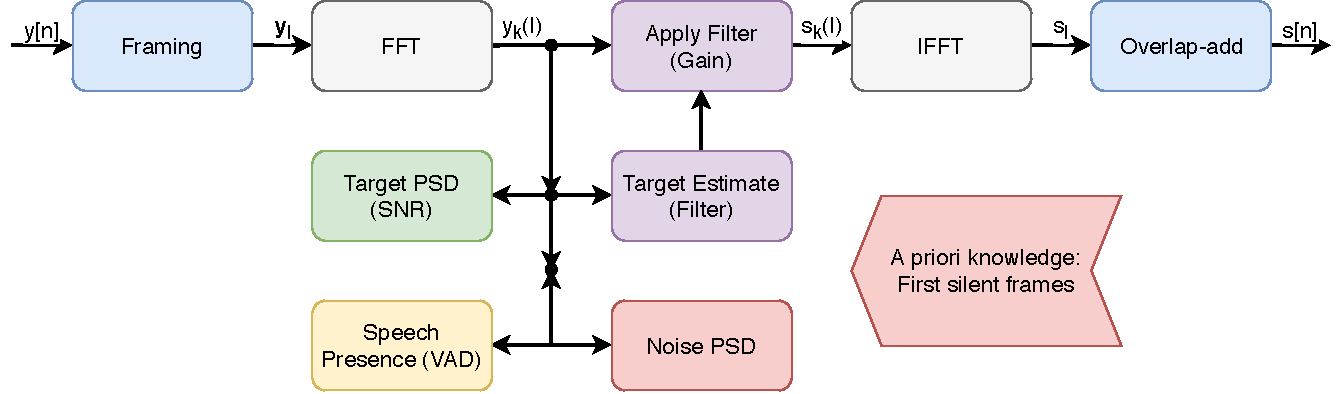
\includegraphics[width=\textwidth]{images/system.pdf}
  \caption{Overview of the system.}
  \label{fig:system}
\end{figure}

This system is focused on a single microphone setup. With a multiple microphone setup, the speech enhancement can be improved upon. Direction estimation and spatial filtering with beamformers can be implemented to filter the unwanted interference and noise from certain directions. This subsystem can be placed before the single microphone speech enhancement system.

The system's functions will be divided into six Sections. The framing and overlap add function will be implemented in Section \ref{sec:framing_overlap_add}. The noise PSD estimation and the source PSD estimation are discussed in Section \ref{sec:noise_estimation} and Section \ref{sec:snr_estimation} respectively. The voice activity detection will be discussed in Section \ref{sec:vad}. With all this information, the target estimation where the filters are designed is discussed in Section \ref{sec:target_estimation}. And lastly, the spatial filtering will be discussed in Section \ref{sec:mm_bf}.
